\documentclass{article}
\usepackage[hmargin=2cm,vmargin=2cm]{geometry}
\usepackage{graphicx}
\usepackage{subcaption}
\usepackage[dvipsnames]{xcolor}
\usepackage{tikz}
\usetikzlibrary{shapes.geometric,shapes.multipart,shapes.symbols,arrows,
	fit,decorations,decorations.pathreplacing,decorations.pathmorphing,calc}
\usepackage{anyfontsize}
\usepackage{chemfig}



\definecolor{PalePineGreen}{RGB}{141,211,199}
\definecolor{PaleSand}{RGB}{255,255,179}
\definecolor{PaleLavender}{RGB}{251,128,114}
\definecolor{PaleRed}{RGB}{251,128,114}
\definecolor{PaleBlue}{RGB}{128,177,211}
\definecolor{PaleOrange}{RGB}{253,180,98}
\definecolor{PaleGreen}{RGB}{179,222,105}
\definecolor{PalePink}{RGB}{252,205,229}
\definecolor{PaleGrey}{RGB}{217,217,217}
\definecolor{PalePurple}{RGB}{188,128,189}
\definecolor{PaleYellowGreen}{RGB}{204,235,197}
\definecolor{PaleYellow}{RGB}{255,237,111}


\definecolor{StrongLightBlue}{RGB}{166,206,227}
\definecolor{StrongBlue}{RGB}{31,120,180}
\definecolor{StrongLightGreen}{RGB}{178,223,138}
\definecolor{StrongGreen}{RGB}{51,160,44}
\definecolor{StrongPink}{RGB}{251,154,153}
\definecolor{StrongRed}{RGB}{227,26,28}
\definecolor{StrongPeach}{RGB}{253,191,111}
\definecolor{StrongOrange}{RGB}{255,127,0}
\definecolor{StrongLavender}{RGB}{202,178,214}
\definecolor{StrongViolet}{RGB}{106,61,154}
\definecolor{StrongSand}{RGB}{255,255,153}
\definecolor{StrongBrown}{RGB}{177,89,40}

	% Define decoration
\pgfdeclaredecoration{lipidleaflet}{initial}
{
	% Place as many segments as possible along the path to decorate
	% the minimum distance between two segments is set to 7 pt.
	\state{initial}[width=\pgfdecoratedpathlength/floor(\pgfdecoratedpathlength/6pt)]
	{
		% Draw the two acyl chains
		\pgfpathmoveto{\pgfpoint{-1pt}{0pt}}
		\pgfpathlineto{\pgfpoint{-1pt}{-10pt}}
		\pgfpathmoveto{\pgfpoint{1pt}{0pt}}
		\pgfpathlineto{\pgfpoint{1pt}{-10pt}}
		% Draw the head group
		\pgfpathmoveto{\pgfpoint{1pt}{0pt}}
		\pgfpathcircle{\pgfpoint{0pt}{2pt}}{2.5pt}
	}
	\state{final}
	{
		\pgfpathmoveto{\pgfpointdecoratedpathlast}
	}
}
\def\centerarc[#1](#2)(#3:#4:#5)% Syntax: [draw options] (center) (initial angle:final angle:radius)
{ \draw[#1] ($(#2)+({#5*cos(#3)},{#5*sin(#3)})$) arc (#3:#4:#5); }

\setchemfig{
	bond offset = 0.75pt,
	double bond sep = 2.5pt,
	bond style = {line width = 0.75pt}
}
\definesubmol\fragment1{
	(-[:#1,0.85,,,draw=none]
	-[::126]-[::-54](=_#(2pt,2pt)[::180])
	-[::-70](-[::-56.2,1.07]=^#(2pt,2pt)[::180,1.07])
	-[::110,0.6](-[::-148,0.60](=^[::180,0.35])-[::-18,1.1])
	-[::50,1.1](-[::18,0.60]=_[::180,0.35])
	-[::50,0.6]
	-[::110])
}

\newsavebox{\mybox}
\sbox{\mybox}{%
	\chemfig{
	!\fragment{-18}
	!\fragment{-90}
	!\fragment{-162}
	!\fragment{-234}
	!\fragment{-306}
	}
}


\begin{document}

\chemfig{
	!\fragment{-18}
	!\fragment{-90}
	!\fragment{-162}
	!\fragment{-234}
	!\fragment{-306}
}

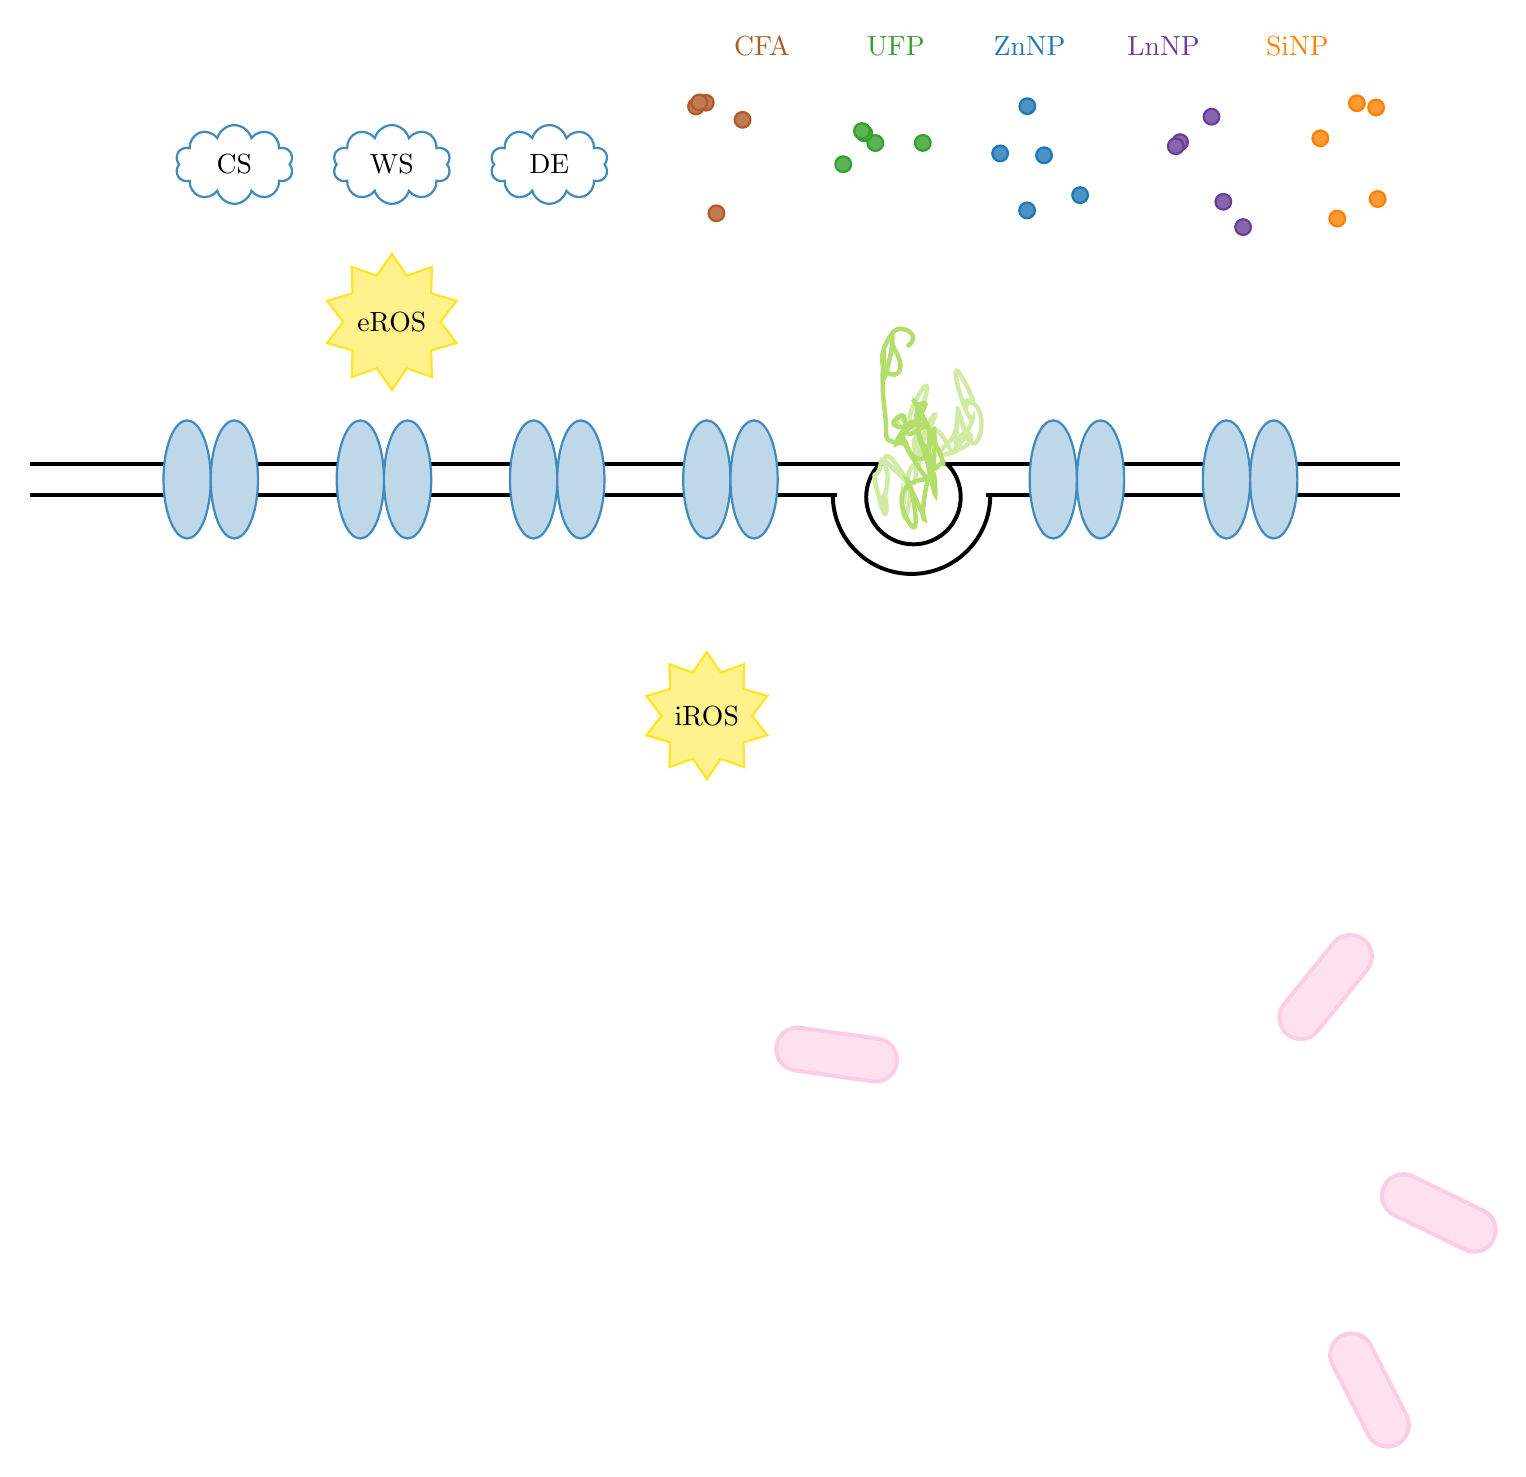
\begin{tikzpicture}
[thick,text centered,
channel/.style={draw=PaleBlue!150,fill=PaleBlue!50,ellipse,minimum width=6mm,minimum height=15mm},
star/.style={draw=PaleYellow!150,fill=PaleYellow!80,shape=star, star points=10, star point
	ratio=1.4,inner sep=0pt,node distance=30mm},
cloud/.style={draw=PaleBlue!150,fill=White,shape=cloud,aspect=2,inner sep=0pt,
	minimum width=15mm,minimum height=10mm,node distance=20mm},
cfa/.style={circle,fill=StrongBrown!80,draw=StrongBrown,inner sep=2pt,node distance=3mm},
ufp/.style={circle,fill=StrongGreen!80,draw=StrongGreen,inner sep=2pt,node distance=3mm},
znnp/.style={circle,fill=StrongBlue!80,draw=StrongBlue,inner sep=2pt,node distance=3mm},
lnnp/.style={circle,fill=StrongViolet!80,draw=StrongViolet,inner sep=2pt,node distance=3mm},
sinp/.style={circle,fill=StrongOrange!80,draw=StrongOrange,inner sep=2pt,node distance=3mm},
textbox/.style={},
fullerene/.pic={
\usebox{\mybox}
},
nucleus/.pic={
	% Contour first
		\pgfmathsetseed{22}
		% Arcs
		\foreach \x in {1.5*#1,2.5*#1,3.5*#1,4.5*#1,5.5*#1}
	{
		% generate U(0,360) random num start points
		\pgfmathsetmacro{\startA}{random(0,360)}
		\pgfmathsetmacro{\gap}{45/\x/#1}
		% Arcs proportional to radius -> gap too -> 45/radius gap arc
		\centerarc[line width=17pt*#1,draw=PalePink,cap=round, rounded corners=1pt](0,0)(\startA:\startA+360-\gap:\x);
	}
	% Connectors
	\foreach \x in {1.5*#1,2.5*#1,3.5*#1,4.5*#1}
	{
		% generate U(0,360) random num start points
		\pgfmathsetmacro{\startC}{random(0,360)}
		\draw[line width=17pt*#1,draw=PalePink,cap=round, rounded corners=1pt]
		(\startC:\x) -- (\startC:\x+#1);
	}
	% Fill second
	\pgfmathsetseed{22}
	% Arcs
	\foreach \x in {1.5*#1,2.5*#1,3.5*#1,4.5*#1,5.5*#1}
	{
		% generate U(0,360) random num start points
		\pgfmathsetmacro{\startA}{random(0,360)}
		\pgfmathsetmacro{\gap}{45/\x/#1}
		% 45/radius gap arc
		% contour arc
		\centerarc[line width=14pt*#1,draw=PalePink!60,cap=round, rounded corners=1pt](0,0)(\startA:\startA+360-\gap:\x);
	}
	% Connectors
	\foreach \x in {1.5*#1,2.5*#1,3.5*#1,4.5*#1}
	{
		% generate U(0,360) random num start points
		\pgfmathsetmacro{\startC}{random(0,360)}
		\draw[line width=14pt*#1,draw=PalePink!60,cap=round, rounded corners=1pt]
		(\startC:\x) -- (\startC:\x+#1);
	}
}]
% Since I need multiple parameters the pic needs to be defined in the long way
\tikzset{
pics/mucus/.style n args={3}{code={
	\pgfmathsetseed{#2}
	\begin{scope}[x=10pt,y=10pt,ultra thick,baseline,cap=round]
	\coordinate (current point) at #1;
	\coordinate (old velocity) at (0,0);
	\pgftransformscale{1.5}
	\coordinate (new velocity) at (rand,rand);
	\pgftransformxscale{0.5}
	\foreach \i in {0,1,...,25}
	{
		\draw[#3] (current point)
		.. controls ++([scale=-1]old velocity) and
		++(new velocity) .. ++(rand,rand)
		coordinate (current point);
		\coordinate (old velocity) at (new velocity);
		\coordinate (new velocity) at (rand,rand);
	}
	\end{scope}
}}
},

% Lipid bilayer
\draw[line width=.5mm]
(-20mm, -98mm) -- (88.5mm, -98mm);
\draw[line width=.5mm]
(96mm, -98mm) -- (154mm, -98mm);
\draw[line width=.5mm]
(-20mm, -102mm) -- (82.5mm, -102mm);
\draw[line width=.5mm]
(101.5mm, -102mm) -- (154mm, -102mm);


\foreach \x in {0,1,2,3,5,6}
{
	\node (ch\x.1)[channel] at (\x*22mm,-100mm){};
	\node (ch\x.2)[channel] at (\x*22mm + 6mm,-100mm){};
}
%mucus vesicle
\draw[line width=.5mm] (88mm,-98mm) arc [start angle=135, delta angle=270, radius=6mm];
\draw[line width=.5mm] (82mm,-102mm) arc [start angle=180, delta angle=180, radius=10mm];

\node(CS)[cloud,above of=ch0.2,yshift=20mm]{CS};
\node(WS)[cloud,right of=CS]{WS};
\node(DE)[cloud,right of=WS]{DE};

\node(eROS)[star,below of=WS,yshift=10mm]{eROS};
\node(iROS)[star,below of=ch3.1]{iROS};

\pic [xshift=0mm,yshift=9mm] {mucus={(92.25mm,-104mm)}{10}{PaleGreen!60}};
\pic [xshift=0mm,yshift=14mm] {mucus={(92.25mm,-104mm)}{12}{PaleGreen}};

\foreach \x in {0,...,4}
{
	\node (cfa\x)[cfa,right of=DE,xshift=rand*6mm+20mm,yshift=rand*8mm]{};
	\node (ufp\x)[ufp,right of=DE,xshift=rand*6mm+40mm,yshift=rand*8mm]{};
	\node (znnp\x)[znnp,right of=DE,xshift=rand*6mm+60mm,yshift=rand*8mm]{};
	\node (lnnp\x)[lnnp,right of=DE,xshift=rand*6mm+80mm,yshift=rand*8mm]{};
	\node (sinp\x)[sinp,right of=DE,xshift=rand*6mm+100mm,yshift=rand*8mm]{};
}

\node (cfatext)[textbox,text=StrongBrown,right of=DE,xshift=17mm,yshift=15mm]{CFA};
\node (ufptext)[textbox,text=StrongGreen,right of=DE,xshift=34mm,yshift=15mm]{UFP};
\node (zmnptext)[textbox,text=StrongBlue,right of=DE,xshift=51mm,yshift=15mm]{ZnNP};
\node (lmnptext)[textbox,text=StrongViolet,right of=DE,xshift=68mm,yshift=15mm]{LnNP};
\node (sinptext)[textbox,text=StrongOrange,right of=DE,xshift=85mm,yshift=15mm]{SiNP};

%cell nucleus
\pic [below of=ch6.1,yshift=-7cm]{nucleus={1}};
\pic [below of=ch6.1,yshift=-7cm]{fullerene};




\end{tikzpicture}

\end{document}
}